% \documentclass[a4paper, 11pt]{article}

% \usepackage{amsmath}
% \usepackage{amssymb}
% \usepackage{amsthm}
% \usepackage{graphicx}
% \usepackage{subfig}

% \title{Tasks 2,4,6 of homework 3}
% \author{}
% \date{}
% \begin{document}
% \maketitle

\section*{Task 2}
As we know, the convergence of the Bernstein polynomial approximation is very slow, therefore we need really high degree polynomials in order to achieve the desired accuracy. We first tried programing the algorithm as it is with the binomial coefficient in its expanded form, that is:
\begin{equation*}
\frac{n!}{k!(n-k)!}
\end{equation*}
However with this approach we only reached an accuracy of 0.0258 as we can not compute directly factorials of large numbers (crashed at $n = 172$). Then we turned to compute the binomial coefficients with MATLAB's built in \texttt{nchoosek} function, this did a better job, lowering the error to 0.008, but this is still not enough. Finally (need to do something).

\section*{Task 4}
We have polynomials of the form:
\begin{equation*}
a_1x^1+a_3x^3+a_5x^5+\ldots+a_{n-1}x^{n-1}
\end{equation*}
This is not a Haar space as we can construct polynomials that have more roots than the Haar space can handle. Consider n = 5, then we have a space of dimension $d=3$.
\begin{equation*}
a_1x^1+a_3x^3
\end{equation*}
By definition, all elements of a Haar space of dimension $n^*+1$ have at most $n^*$ roots. In our case, $n^*+1 = 3$ thus, all elements of the space have to have at most $n^*=2$ roots. However let us construct a polynomial with 3 roots. We want a polynomial of the form $(x-x_1)(x-x_2)(x-x_3)$. Expanding this expression we get:
\begin{equation*}
x^3-x^2(x_3+x_2+x_1)+x(x_2x_3+x_1x_3+x_1x_2)-x_1x_2x_3
\end{equation*}
As we want the $x^2$ and the independent term to be gone we get a system of equations:
\begin{align*}
x_3+x_2+x_1 &= 0 \\
x_1x_2x_3 &= 0
\end{align*}
Let $x_3 = 0$, then we get $x_1 = -x_2$, for example let $x_1 = 1$ then we have:
\begin{equation*}
p(x) = x(x-1)(x+1) = x^3-x
\end{equation*}
\qed

\section*{Task 6}
The operator is not linear. Let $f(x) = \sin (x), g(x) = \cos (x)$ and consider the space $\mathcal{P}_0 \subset \mathcal{C}[0, \pi/2]$. It is easy to see that the best minimax approximation to both of these functions is $p(x) = 1/2$ as it satisfies the characterization theorem. However if we take $f(x)+g(x)$ we get that the best minimax approximation is $p(x) = \sin(\pi/4)+\cos(\pi/4)>1$. thus the property:
\begin{equation*}
X(f+g) = X(f) + X(g)
\end{equation*}
is not fulfilled.
\begin{figure}[h]
\centering 
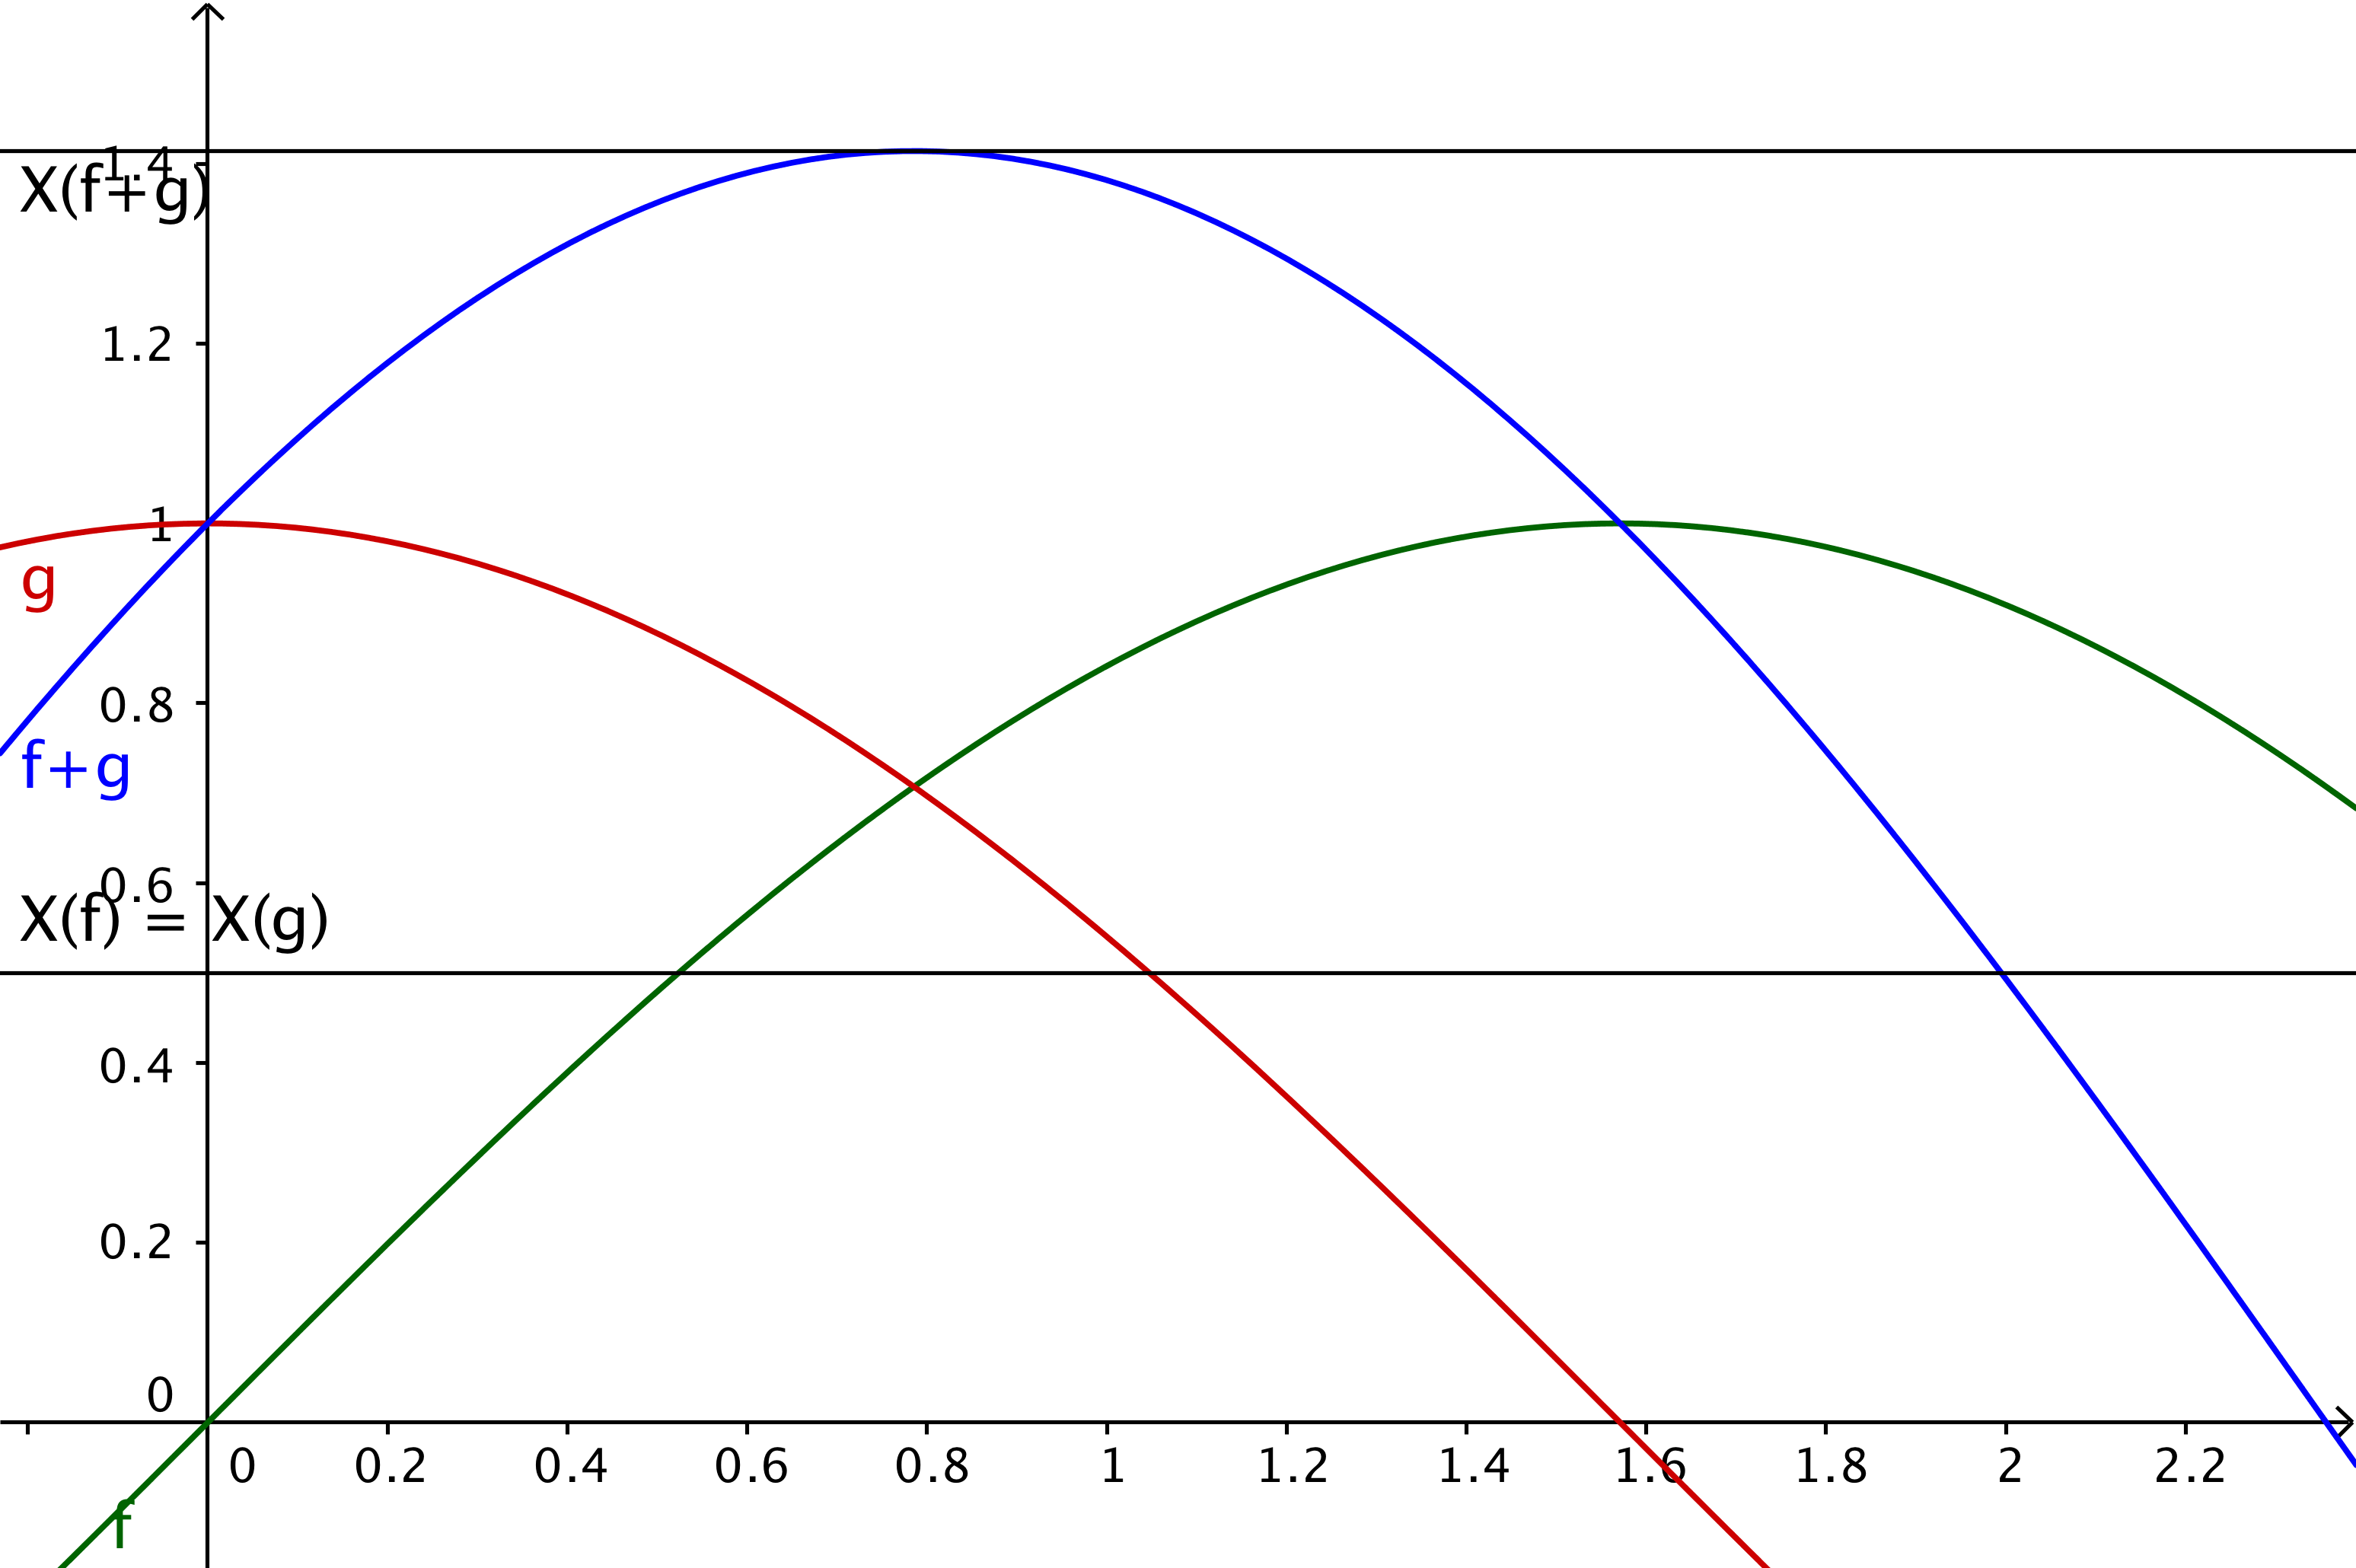
\includegraphics[scale = 0.5]{figtask6.png}
\caption{Plot of the functions and their best minimax approximations}
\label{figtask6}
\end{figure}
\qed
\end{document}

%%% Local Variables:
%%% mode: latex
%%% TeX-master: "report"
%%% End:
